% Vertical (portrait) architecture figure for the A0 poster.
% Same content as REPORT_v6 Figure 1, re-proportioned: the top-to-bottom
% pipeline is the dominant axis; the support rail is narrow.
\documentclass[tikz,border=2mm]{standalone}
\usetikzlibrary{positioning,arrows.meta,calc}
\begin{document}
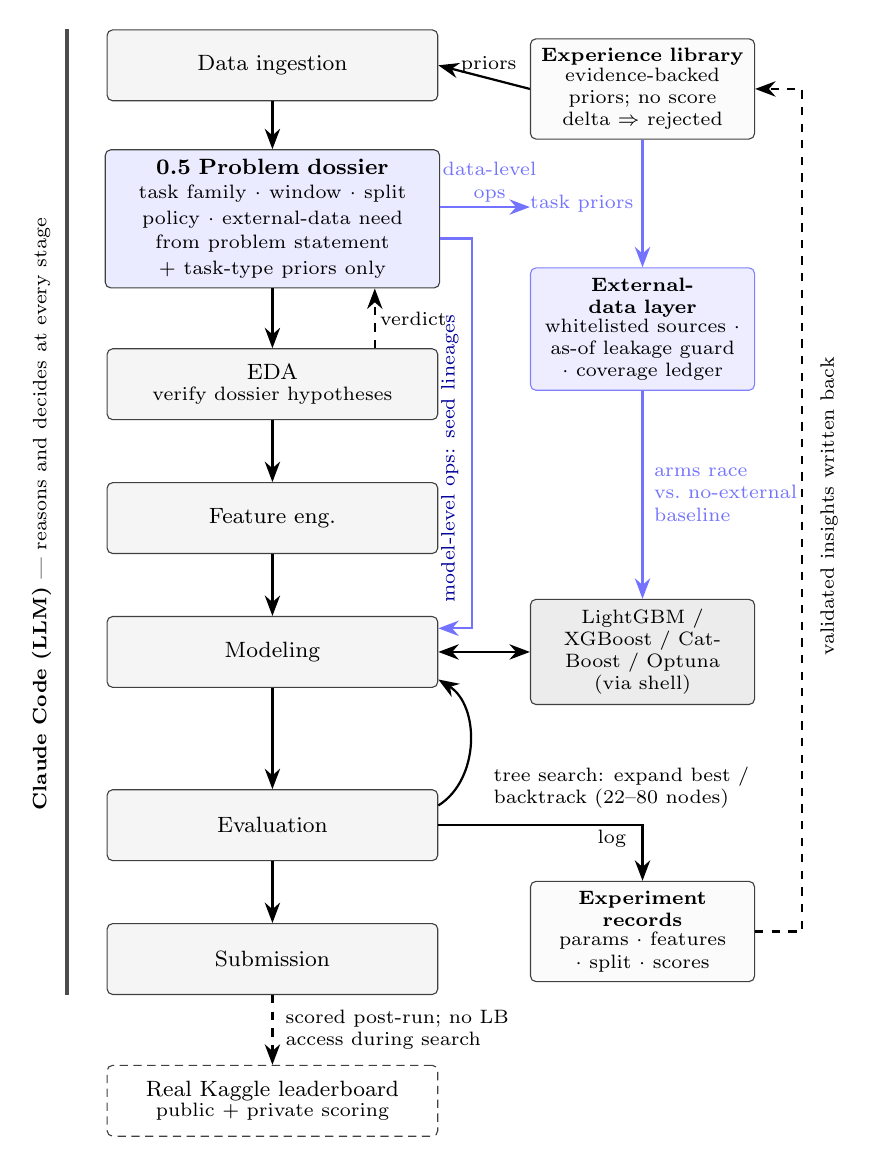
\begin{tikzpicture}[
  font=\footnotesize,
  stage/.style={draw=black!75, rounded corners=2pt, align=center, inner sep=3.5pt,
                fill=gray!8, minimum height=9mm, minimum width=42mm},
  supp/.style={draw=black!75, rounded corners=2pt, align=center, inner sep=3.5pt,
               fill=gray!3, text width=26mm, font=\scriptsize},
  injbox/.style={supp, fill=blue!7, draw=blue!50},
  toolbox/.style={supp, fill=gray!15},
  arr/.style={-{Stealth[length=2.6mm]}, thick},
  barr/.style={arr, blue!55},
  darr/.style={arr, dashed},
  lab/.style={font=\scriptsize, inner sep=1.5pt}
]
% ----- main pipeline (top -> bottom, the dominant axis) -----
\node[stage]              (s1)  at (0,0)     {Data ingestion};
\node[stage, fill=blue!8, text width=40mm] (s05) at (0,-1.95)
  {\textbf{0.5 Problem dossier}\\[-1pt]
   {\scriptsize task family $\cdot$ window $\cdot$ split policy $\cdot$ external-data need}\\[-1pt]
   {\scriptsize from problem statement + task-type priors only}};
\node[stage]              (s2)  at (0,-4.05) {EDA\\[-2pt]{\scriptsize verify dossier hypotheses}};
\node[stage]              (s3)  at (0,-5.75) {Feature eng.};
\node[stage]              (s4)  at (0,-7.45) {Modeling};
\node[stage]              (s5)  at (0,-9.65) {Evaluation};
\node[stage]              (s6)  at (0,-11.35) {Submission};
\foreach \a/\b in {s1/s05, s05/s2, s2/s3, s3/s4, s4/s5, s5/s6}{\draw[arr] (\a) -- (\b);}
\draw[darr] ([xshift=13mm]s2.north) -- node[lab, right]{verdict} ([xshift=13mm]s05.south);
% ----- endpoint: the real leaderboard -----
\node[stage, densely dashed, fill=white] (lb) at (0,-13.15)
  {Real Kaggle leaderboard\\[-2pt]{\scriptsize public + private scoring}};
\draw[darr] (s6) -- node[lab, anchor=west, xshift=1mm, align=left]
  {scored post-run; no LB\\access during search} (lb);
% ----- LLM band, left edge -----
\draw[line width=1.2pt, black!70]
  ([xshift=-5mm]s6.south west) -- ([xshift=-5mm]s1.north west);
\node[lab, rotate=90, anchor=south] at (-2.75,-5.7)
  {\textbf{Claude Code (LLM)} --- reasons and decides at every stage};
% ----- tree-search loop -----
\draw[arr] ([yshift=2.5mm]s5.east) to[out=32, in=-32] ([yshift=-3.5mm]s4.east);
\node[lab, anchor=north west, align=left] at (2.75,-8.85)
  {tree search: expand best /\\backtrack (22--80 nodes)};
% ----- right rail (narrow) -----
\node[supp]    (lib)   at (4.7,-0.3)
  {\textbf{Experience library}\\[-1pt] evidence-backed priors; no score delta $\Rightarrow$ rejected};
\node[injbox]  (ext)   at (4.7,-3.35)
  {\textbf{External-data layer}\\[-1pt] whitelisted sources $\cdot$ as-of leakage guard $\cdot$ coverage ledger};
\node[toolbox] (tools) at (4.7,-7.45)
  {LightGBM / XGBoost / CatBoost / Optuna\\ (via shell)};
\node[supp]    (rec)   at (4.7,-11.0)
  {\textbf{Experiment records}\\[-1pt] params $\cdot$ features $\cdot$ split $\cdot$ scores};
% ----- connections -----
\draw[arr]  (lib.west) -- node[lab, above, align=center, pos=0.45]{priors} (s1.east);
\draw[barr] (lib.south) -- node[lab, anchor=east, xshift=-0.5mm]{task priors} (ext.north);
\draw[barr] ([yshift=1.5mm]s05.east) -- node[lab, above, pos=0.55, align=center]{data-level\\ops}
  ([yshift=1.5mm]ext.west |- s05.east);
\draw[barr] ([yshift=-2.5mm]s05.east) -- ++(4mm,0) |- ([yshift=3mm]s4.east);
\node[lab, rotate=90, anchor=south, blue!60!black] at (2.42,-5.0)
  {model-level ops: seed lineages};
\draw[barr] (ext.south) -- node[lab, anchor=west, xshift=0.8mm, align=left]
  {arms race\\vs.\ no-external\\baseline} (tools.north);
\draw[arr, {Stealth[length=2.6mm]}-{Stealth[length=2.6mm]}] (s4.east) -- (tools.west);
\draw[arr]  (s5.east) -- node[lab, below, pos=0.85]{log} (rec.north |- s5.east) -- (rec.north);
% ----- dashed write-back, far right -----
\draw[darr] (rec.east) -- ++(6mm,0) |- (lib.east);
\node[lab, rotate=90, anchor=north] at (6.9,-5.6)
  {validated insights written back};
\end{tikzpicture}
\end{document}
